
\chapter{Số bội giác của kính lúp}

\section{Lý thuyết trọng tâm}

\subsection{Số bội giác}
\subsubsection{Khái niệm số bội giác}
Các dụng cụ quang học đều có tác dụng tạo ảnh với góc trông ảnh lớn hơn góc trông vật nhiều lần. Đại lượng đặc trưng cho tác dụng này là số bội giác.

Công thức:
\begin{equation}
G=\dfrac{\alpha}{\alpha_0}\approx \dfrac{\tan \alpha}{\tan \alpha_0},
\end{equation}
trong đó,
\begin{itemize}
	\item $\alpha$ là góc trong ảnh qua kính (radian),
	\item $\alpha_0$ là góc trông trực tiếp vật có giá trị lớn nhất trong từng trường hợp (radian),
	\item $G$ là số bội giác. 
	
\end{itemize}

\subsubsection{Số bội giác của kính lúp khi ngắm chừng vô cực}

Số bội giác: $$G_\infty=\dfrac{\alpha}{\alpha_0}\approx \dfrac{\tan \alpha}{\tan \alpha_0}.$$ 

Khi quan sát vật AB trực tiếp bằng mắt: $$\tan \alpha_0=\dfrac{\text{AB}}{\text{OC}_\text{c}}.$$
\begin{center}
	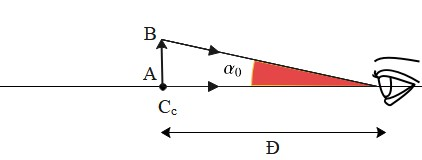
\includegraphics[scale=0.8]{../figs/VN11-PH-41-L-029-2-h47.jpg}
\end{center}


Khi quan sát vật qua kính lúp: $$\tan \alpha=\dfrac{\text{AB}}{f}.$$
\begin{center}
	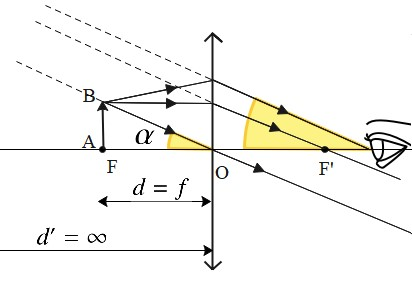
\includegraphics[scale=0.8]{../figs/VN11-PH-41-L-029-2-h48.jpg}
\end{center}

Do đó: $$G_\infty=\dfrac{\tan \alpha}{\tan \alpha_0}=\dfrac{\text{AB}}{f}\cdot \dfrac{\text{OC}_\text{c}}{\text{AB}}$$
hay 
\begin{equation}
G_\infty=\dfrac{\text{OC}_\text{c}}{f}=\dfrac{\text{Đ}}{f},
\end{equation}
trong đó,
\begin{itemize}
	\item $\text{Đ}$ là khoảng cực cận của mắt,
	\item $f$ tiêu cự của kính lúp,
	\item $G_\infty$ là số bội giác khi ngắm chừng ở vô cực. 
	
\end{itemize}

\luuy{Người ta thường lấy khoảng cực cận là $\text{OC}_\text{c}=25\ \text{cm}$. Khi sản xuất kính lúp, người ta ghi giá trị của $G_\infty$ ứng với khoảng cực cận này trên kính.
	
Ví dụ : Các kính có kí hiệu 3x, 6x, 8x,... sẽ có tiêu cự tương ứng là 
$\dfrac{25}{3}\ \text{cm}, \ \dfrac{25}{6}\ \text{cm}, \ \dfrac{25}{8}\ \text{cm},...$ Chúng có khả năng làm cho góc trông ảnh qua kính lớn hơn ba lần, sáu lần, tám lần,... góc trông trực tiếp vật.} 

\subsubsection{Số bội giác của kính lúp khi ngắm chừng ở cực cận}
Ta đã biết,  $\tan \alpha_0=\dfrac{\text{AB}}{\text{OC}_\text{c}}$.

\begin{center}
	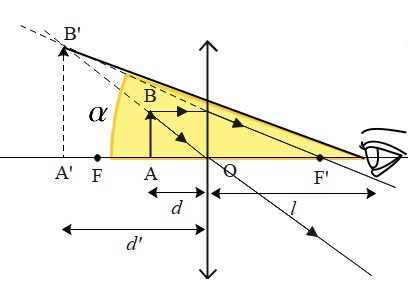
\includegraphics[scale=0.8]{../figs/VN11-PH-41-L-029-2-h49.jpg}
\end{center}


Gọi $l$ là khoảng cách từ mắt đến kính lúp và $d’$ là khoảng cách từ ảnh A’B’ đến kính $(d’<0)$:
	\begin{eqnarray*}
			\tan \alpha &=&\dfrac{\text{A'B'}}{|d'|+l}\\
			G=\dfrac{\tan \alpha}{\tan \alpha_0}&=&\left(\dfrac{\text{A'B'}}{\text{AB}}\cdot \dfrac{\text{Đ}}{|d'|+l} \right)
	\end{eqnarray*}
hay 
\begin{equation}
G=|k|\cdot \dfrac{\text{Đ}}{|d'|+l},
\end{equation}
trong đó, $|k|$ là độ lớn của số phóng đại ảnh cho bởi kính lúp.

Khi ngắm chừng ở cực cận, ta có: $|d'|+l=\text{Đ}$, do đó:
\begin{equation}
G_\text{c}=|k|.
\end{equation}


\section{Bài tập }
\begin{dang}{Ngắm chừng ở vô cực}
\end{dang}
\textbf{Phương pháp giải}

Sử dụng công thức thấu kính: $D=\dfrac{1}{f}=\dfrac{1}{d}+\dfrac{1}{d'}$ 

Sử dụng công thức tính số bội giác khi ngắm chừng vô cực
\begin{equation}
G_\infty=\dfrac{\text{OC}_\text{c}}{f}=\dfrac{\text{Đ}}{f},
\end{equation}
trong đó,
\begin{itemize}
	\item $\text{Đ}$ là khoảng cực cận của mắt,
	\item $f$ tiêu cự của kính lúp,
	\item $G_\infty$ là số bội giác khi ngắm chừng ở vô cực. 
\end{itemize}

Khoảng cực cận Đ của mắt thường là $25\ \text{cm}$.

\vspace{1em}

\vidu{3}{
Một người có khoảng nhìn rõ từ 25 cm đến vô cực, quan sát một vật nhỏ qua kính lúp có độ tụ $D = 20\ \text{dp}$ trong trạng thái ngắm chừng ở vô cực. Độ bội giác của kính là
\begin{mcq}
	\item 2 dp.
	\item 4 dp.
	\item 5 dp.
	\item 7 dp.
\end{mcq}}{
\begin{center}
	\textbf{Hướng dẫn giải:}
\end{center}

{ Tiêu cự của kính lúp là $f=\dfrac{1}{D}= \text{0,05}\ \text{m} = 5 \ \text{cm}$.
	
Khoảng cực cận là $\text{Đ}=\text{OC}_\text{c}=25 \ \text{cm}$.

Số bội giác của kính lúp khi ngắm chừng ở vô cực là

 $G_\infty=\dfrac{\text{OC}_\text{c}}{f}=\dfrac{\text{Đ}}{f}=5 \ \text{cm}$.
		 
\textbf{	Đáp án: C.}
}

}
\begin{dang}{Ngắm chừng ở cực cận}
\end{dang}
\textbf{Phương pháp giải}

Sử dụng công thức thấu kính: $D=\dfrac{1}{f}=\dfrac{1}{d}+\dfrac{1}{d'}$ 

Sử dụng công thức tính số bội giác khi ngắm chừng ở vị trí bất kỳ: 
\begin{equation}
G=|k|\cdot \dfrac{\text{Đ}}{|d'|+l},
\end{equation}
trong đó, $|k|$ là độ lớn số phóng đại của ảnh cho bởi kính lúp.

Khi ngắm chừng ở cực cận, ta có: $|d'|+l=\text{Đ}$, do đó:
\begin{equation}
G_\text{c}=|k|.
\end{equation}


\viduii{3}{

Một kính lúp có độ tụ 50 dp. Mắt có điểm cực cận cách mắt 20 cm đặt tại tiêu điểm ảnh của kính để nhìn vật AB dưới góc trông ảnh bằng $\text{0,05}\ \text{rad}$, mắt ngắm chừng ở vô cực.
\begin{enumerate}
	\item Xác định chiều cao của vật.
	\item Đặt mắt cách kính lúp 5cm và ngắm chừng ở điểm cực cận. Tính số bội giác.
\end{enumerate}}
{\begin{center}
	\textbf{Hướng dẫn giải:}
\end{center}

 
	\begin{enumerate}
	\item Xác định chiều cao của vật.
	
	Tiêu cự của kính lúp là $f=\dfrac{1}{D}=2 \ \text{cm}$.
	
	Khi ngắm chừng vô cực: 
	
	$\tan \alpha=\dfrac{\text{AB}}{f}\Rightarrow \text{AB}=f\cdot \tan \alpha=\text{0,1} \ \text{cm}$.	
	\item 	Khi ngắm chừng cực cận:
	
	Khoảng cực cận là $\text{Đ}=\text{OC}_\text{c}=20 \ \text{cm}$.
	
    $|d'|=\text{Đ}-l=15\ \text{cm}\Rightarrow d'=-15\ \text{cm}$ (do A'B' là ảnh ảo).
    
    $\dfrac{1}{f}=\dfrac{1}{d}+\dfrac{1}{d'}\Rightarrow d=\dfrac{30}{17}\ \text{cm} $.
    
    	$G_\text{c}=|k|=\left|-\dfrac{d'}{d} \right|=\text{8,5}\ \text{dp}$. 
	
\end{enumerate}

}

\viduii{3}{\textbf{ [TN THPT 2020 - Mã đề 205] }
Một người dùng kính lúp để quan sát vật AB có chiều cao $11\ \mu m$  được đặt vuông góc với trục chính (A nằm trên trục chính). Khi mắt đặt sát sau kính và ngắm chừng ở điểm cực cận thì góc trông ảnh của vật qua kính lúp là $\text{3,19}\cdot 10^{-4}\  \text{rad}$. Biết mắt người này có khoảng cực cận $\text{Đ} = 25\ \text{cm}$. Tiêu cự của kính lúp bằng
\begin{mcq}
	\item $\text{4,5}\ \text{cm}$.
	\item $\text{4}\ \text{cm}$.
	\item $\text{5,5}\ \text{cm}$.
	\item $\text{5}\ \text{cm}$.
\end{mcq}}
{\begin{center}
	\textbf{Hướng dẫn giải:}
\end{center}

{ \begin{center}
		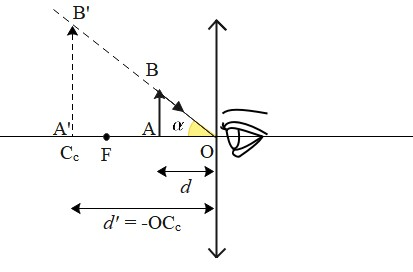
\includegraphics[scale=0.8]{../figs/VN11-PH-41-L-029-2-h50.jpg}
	\end{center}

Theo đề bài, góc trông ảnh $\alpha=\text{3,19}\cdot 10^{-4}\  \text{rad}$.
	
$d$ là khoảng cách từ vật đến thấu kính.

Vì kính đặt sát mắt nên: $\tan \alpha=\dfrac{\text{AB}}{d}\Rightarrow d=\text{0,0345}\ \text{m}=\text{3,45}\ \text{cm}$.

Khi ngắm chừng ở cực cận thì ảnh ảo của vật nằm ở điểm cực cận. 

Tức là $d'=-\text{OC}_{\text{c}}=-\text{Đ}=-25\ \text{cm}$.

Công thức thấu kính: $\dfrac{1}{f}=\dfrac{1}{d}+\dfrac{1}{d'}\Rightarrow f =4\ \text{cm}$.

\textbf{Đáp án: B.}
	
	
}

 
}